\chapter{Pebble Modeling: Discrete Element Method} \label{modeling-DEM}
%%%%%%%%%%%%%%%%%%%%%%%%%%%%%%%%%%%%%%%%%%%%%%%%%%%%%%%%%%%%%%%%%%%%%%%%%%%%%%%%%%%%%%%%%%%%%%
%%%%%%%%%%%%%%%%%%%%%%%%%%%%%%%%%%%%%%%%%%%%%%%%%%%%%%%%%%%%%%%%%%%%%%%%%%%%%%%%%%%%%%%%%%%%%%
This chapter presents the motivations and background of this study. First, it discusses energy usage in our society and the inevitable production of waste mechanical and thermal energies and their ubiquitous nature. This is followed by a brief discussion of common methods of converting ambient mechanical energy and waste heat into useful electrical energy. This chapter concludes with the objectives of this study and the scope of the document.



\subsection{Background}
\label{sec:dem-intro}

The observable, macroscopic behavior of particulate, or granular, systems is a complex function of the multitude of particle-scale interactions. Historically, empirical relationships have been used to describe these systems as if a continuous media. But with the advent of the discrete element method by Cundall and Strack\cite{Cundall1979} and the acceleration of computing power, it became practical to investigate these particulate systems at the particle scale. With the discrete element method, we track all the particles in the system in a Lagrangian manner. In the ensemble, the kinematics of each particle is tracked and updated based on balances (or imbalances) of forces or energy acting upon the particle.

Experiments on packed beds are generally limited to measurements of statistically averaged, macroscopic responses. Unlike continuous materials, packed beds as yet can not be described by any State. For instance, with an ideal gas if we know two properties such as temperature or pressure, the State of the gas is known and its behavior predicted. Two packed beds with the same temperature, packing fraction, average particle diameter, and stress state may react wildly different. As researchers we create empirical fits to data on the particular packed bed under investigation but then might have to dubiously apply the relationships to beds of different packing states. 

DEM is emerging as a reliable method to remove speculation about the internal state of the packed bed as the simulations provide valuable information on the dynamics of particle interactions and how they relate to the macroscopic responses that are measured experimentally.

In this chapter we will lay out the formulas governing interaction of particles in the DEM framework, the methods of computation, and the code used for implementation. In \cref{sec:dem-stability}, we will use the derivation of the Hertz contact law described in \cref{sec:hertz-theory} to argue for a technique of accelerating the computational time without loss of physics via proper scaling of physical parameters. Lastly, in \cref{sec:dem-studies-effective-conductivity}, we use our DEM tools to investigate the thermo physics of representative packed beds for solid breeders in fusion reactors.

\subsection{Particle Dynamics}\label{sec:particle-dynamics}

The particles in our system are allowed translational and rotational degrees of freedom. In a packed bed, we can restrict our attention to local forces between particles; neglecting, say, non-contact forces such as van der Waals or electrostatic forces. In the first construct of momentum and temperature consideration, I will treat the particles as if in a vacuum. However a derivation of fluid interaction forces will be given in \cref{sec:modeling-cfd-dem}.



%~~~~~~~~~~~~~~~~~~~~~~~~~~~~~~~~~~~~~~~~~~~~~~~~~~~~~~~~~~~~~~~~~~~~
\subsubsection{Particle Kinematics}

Assuming we know the contact forces acting upon particle $i$, Newton's equations of motion are sufficient to describe the kinematics of the particle. For the translation and rotational degrees of freedom, the equations are:,
\begin{subequations}
\label{eq:newtons-second}
\begin{align}
	m_i  \ddt{\vec{r}_i}   & = m_i\vec{g} + \vec{f}_i \label{eq:newton-translational} \\
	I_i\dt{\vec{\omega}_i} & = \vec{T}_i \label{eq:newton-rotational}
\end{align}
\end{subequations}
where $m_i$ is the mass of this particle, $\vec{r}_i$ its location in space, $\vec{g}$ is gravity, $I_i$ is the particle's moment of inertia, and $\vec{\omega}_i$ its angular velocity.

The net contact force, $\vec{f}_i$, represents the sum of the normal and tangential forces from the total number of contacts, $Z$, acting on this particle.
\begin{equation}
 	\vec{f}_i = \sum_{j=1}^{Z} \vec{f}_{n,ij} + \vec{f}_{t,ij}
 \end{equation} 
and the net torque, $\vec{T}_i$, is similarly,
\begin{equation}
	\vec{T}_i = -\frac{1}{2}\sum_{j=1}^{Z} \vec{r}_{ij} \times \vec{f}_{t,ij}
\end{equation}

When Cundall and Strack first proposed the discrete element method, they used a linear spring-dashpot structure which saw the normal and tangential forces written as,
\begin{subequations}
\label{eq:dem-forces}
\begin{align}
	\vec{f}_{n,ij} &= k_{n,ij} \delta_{n,ij}\vec{n}_{ij} - \gamma_{n,ij} \vec{u}_{n,ij} 	\label{eq:normal-force} \\
	\vec{f}_{t,ij} &= k_{t,ij} \delta_{t,ij}\vec{t}_{ij} - \gamma_{t,ij} \vec{u}_{t,ij} 	\label{eq:tangential-force}
\end{align}
\end{subequations}
where, in the first model of Cundall and Strack, the stiffness coefficients $k$ were constants and the local damping coefficients $\gamma$ were proportional to them, $\gamma \propto k$, to allow dissipation of energy and the system to reach an equilibrium. The relative normal and tangential velocities, respectively, are decomposed from the particle velocities,

\begin{subequations}
\label{eq:dem-velocities}
\begin{align}
	\vec{u}_{n,ij} &= (-(\vec{u}_i-\vec{u}_j)\cdot\vec{n}_{ij})\vec{n}_{ij} \\
	\vec{u}_{t,ij} &= (-(\vec{u}_i-\vec{u}_j)\cdot\vec{t}_{ij})\vec{t}_{ij}
\end{align}
\end{subequations}
with the unit vector $\vec{n}_{ij}$ pointing from particle $j$ to $i$

Similarly to the approach of Hertz (see \cref{sec:hertz-theory}), the surfaces of the two particles are allowed to virtually pass through each other (no deformation) resulting in normal and tangential overlaps of,

\begin{subequations}
\label{eq:dem-overlaps}
\begin{align}
	\delta_{n,ij} &= (R_i + R_j) - (\vec{r}_i -\vec{r}_j)\cdot \vec{n}_{ij} \\
	\delta_{t,ij} &= \int_{t_{c,0}}^{t} \vec{u}_{t,ij}\,\mathrm{d}\tau 
\end{align}
\end{subequations}
where the fictive tangential overlap, $\delta_{t,ij}$, is truncated to so the tangential and normal forces obey Coulomb's Law, $\vec{f}_{t,ij} \le \mu_i \vec{f}_{n,ij}$ with $\mu$ as the coefficient of friction of the particle.

The result is a relatively simple approach of calculating the interaction forces between particles with Eq.~\ref{eq:dem-forces} based on the kinematics of velocity and position of the interacting particles from Eq.~\ref{eq:dem-velocities} and Eq.~\ref{eq:dem-overlaps}, respectively. As the DEM evolved and drew the attention of more researchers, more complex formulas governing the spring-dashpot coefficients of Eq.~\ref{eq:dem-forces} emerged. But the core approach remained the same and the models all fall into the same family of so-called `soft particle' models of DEM. A well-composed summary of the different DEM force models is given by Zhu\etal\cite{Zhu2007}.

The method used in this work fits into the computational skeleton of Cundall and Strack's method but with non-linear spring-dashpot coefficients defined by simplified Hertz-Mindlin-Deresiewicz model. In this model, the normal-direction stiffness coefficient of Eq.~\ref{eq:normal-force} is based on the Hertzian contact law (derived explicitly in \cref{sec:hertz-theory}). The tangential-direction stiffness coefficient follows from Brilliantov.\cite{Brilliantov1996, Zhu2007, Langston1995} Together, the spring coefficients are,
\begin{subequations}
\begin{align}
	k_{n,ij} &= \frac{4}{3}E_{ij}^*\sqrt{R_{ij}^*\delta_{n,ij}} \\
	k_{t,ij} &= 8 G_{ij}^*\sqrt{R_{ij}^*\delta_{t,ij}}
\end{align}
\end{subequations}
where $E_{ij}^*$ is the pair Young's modulus, $G_{ij}^*$ is the pair bulk modulus, and $R_{ij}^*$ is the relative radius. The terms are defined as,
\begin{subequations}
\begin{align}
	\frac{1}{E^*} &= \frac{1-\nu_1^2}{E_1} + \frac{1-\nu_2^2}{E_2} \\
	\frac{1}{R^*} &= \frac{1}{R_1} + \frac{1}{R_2} \\
	\frac{1}{G^*_{ij}} &= \frac{2(2+\nu_i)}{E_i} + \frac{2(2+\nu_j)}{E_j}
\end{align}
\end{subequations}

The damping coefficients, $\gamma$, arise to account for the energy dissipated from the collision of two particles\cite{DiRenzo2004, Tsuji1992, Tsuji1993}. Whether the damping coefficient is local or global and the exact form of the coefficient is more important for loosely confined granular systems and dictates the way the system approaches an equilibrium state\cite{Makse2004}. For the case of our tightly packed pebble beds, it suffices to use the efficient form of\cite{Dippel1996, Makse2004, Brilliantov1996, Zhang2005, Zhu2007},
\begin{subequations}
\begin{align}
	\gamma_n &= \sqrt{5}\beta_\text{diss}\sqrt{m^*k_{n,ij}} \\
	\gamma_t &= \sqrt{\frac{10}{3}}\beta_\text{damp}\sqrt{k_{t,ij} m^*}
\end{align}
\end{subequations}
with $\beta_\text{damp}$ as the damping ratio, and the pair mass, $\frac{1}{m^*} = \frac{1}{m_i} + \frac{1}{m_j}$. For a stable system with $\beta_\text{damp} < 1$, the damping ratio is related to the coefficient of restitution, $e$, as
\begin{equation}
	\beta_\text{diss} = -\frac{\ln{e}}{\sqrt{\ln^2{e}+\pi^2}}
\end{equation}

Systems are therefore well-defined after specifying the few material properties of $E$, $\nu$, $\rho$, and $R_p$ and the interaction properties of $\mu$ and $e$.

Having expressed the contact mechanics of the discrete element method, we now must integrate the kinematic equations of the particles to resolve their evolutions. The most common means of marching in time with DEM is the velocity-Verlet algorithm\cite{Kruggel-Emden2008}. In this algorithm, Eqs.~\ref{eq:newtons-second} are integrated with half-steps in velocity, full steps in position, and then finally the full step in velocity. In practice, the two half-steps in velocity are often compressed into a single, full step. The computational time integration steps are given in explicit detail in \cref{sec:dem-stability}. Owing to the explicit nature of the velocity-Verlet algorithm, stability is a constant concern with DEM simulations. Stable, critical time steps and means of circumventing unreasonably small time steps will also be addressed in \cref{sec:dem-stability}.

Lastly, in this work, I occasionally required a fully quiesced bed to act as a starting point or demarcate a mechanically steady-state bed. To determine when this occurs, the total kinetic energy of the entire ensemble is monitored and a packed bed is considered to have completely settled once the kinetic energy of the system is less than $10^{-8}$. A similar process was independently determined in a similar matter in the work of Ref.~\cite{Silbert2002}. 
\section{Granular heat transfer}\label{sec:dem-heat-transfer}

In an analogous way we handled the momentum of every particle in DEM with Newton's laws of motion, the Lagrangian tracking of energy of each particle is obtained via the first law of thermodynamics. We treat each particle is a single distinct object and thus do not consider any internal temperature gradients (a point which we alluded to in \cref{sec:ht-jeffreson-correction}). The temperature of particle $i$ is governed by

\begin{equation}\label{eq:thermoFirstLaw}
	\rho_iV_iC_i\frac{\mathrm{d}T_i}{\mathrm{d}t} = Q_{s,i} + Q_{i}
\end{equation}

where $\rho$, $V$, and $C$ are the density, volume, and the specific heat of the solid, respectively. Heat generation inside the particle is input with $Q_{s}$ and the total heat transferred to/from particle $i$ via conduction to all, $Z$, neighboring particles,

\begin{equation}
	Q_i = \sum_{j=1}^Z Q_{ij}
\end{equation}

The conductive heat transfer to neighboring particles comes from the inter-particle conduction formulas we derived in \cref{sec:ht-pebble-conduction}, given in Eq.~\ref{eq:pebble-conduction-heat-transfer} with conductance of Eq.~\ref{eq:cheng-modification-batchelor}. They are repeated here for reference,

\begin{equation*}
	Q_{ij} = H_c(T_i - T_j)
\end{equation*} 

and

\begin{equation}\label{eq:dem-conductance}
	H_c= 2k^*\left[\frac{3F_{n,ij}R^*}{4E^*}\right]^{1/3}
\end{equation}

\subsection{Thermal expansion}
The stresses predicted to act upon the solid breeder volume during operation of the fusion reactor arise from the differential rate of thermal expansion from the highly heated ceramic volume and the relatively cool structural container. Moreover, thermal creep motion is observed in pebble beds\cite{Tanigawa:2010cr, Vargas2007, Chen2009, Divoux2008} and is behavior we must capture in our model. Both of those phenomena can be traced to the thermal expansion of individual particles in the ensemble. Therefore, we introduce a thermal expansion formula that updates the diameter of each particle after a chosen amount of timesteps,

\begin{equation}
	d_i = d_{0,i}\left[1+\beta_i\left(T_i - T_\text{ref}\right)\right]
\end{equation}

where $\beta_i$ is the thermal expansion coefficient (in units of \si{1/K}), $T_i$ is the temperature of the pebble at the current step, and $d_{0,i}$ is the diameter of the pebble at temperature $T_\text{ref}$.


\section{Stability study}\label{sec:dem-stability}
As mentioned when the integration algorithm was introduced in \S\ref{sec:particle-dynamics}, the velocity-Verlet algorithm is a computationally efficient, second-order accurate means of updating the kinematics of all the particles in the ensemble\cite{Kruggel-Emden2008}. The timestep of the integration, however, must often be very small to ensure that it is less than the time taken for a pressure wave to propagate through the particle. The timestep is further constrained by the quasistatic assumption used to derive the Hertzian contact force such that inertial and relaxation effects may be neglected\cite{Brilliantov1996}. We will also show that, in order to avoid heat energy to propagate further than a single pebble during a single timestep, the thermal timestep requirement is orders of magnitude larger than the mechanical timestep equivalent. And that the overall minimum timestep is thus driven by the mechanical stability.

In tandem with the requirement on very small timestep, the thermal time-constants in the ceramic breeder zones can be many hundreds of seconds. These two conditions seem to conspire to force an unacceptably large requirement on the number of timesteps for a thermal DEM simulation and thus make numerical experiments impractical.

In this section we will analyze the calculation of a critical timestep based on the speed of a Rayleigh wave propagating along the surface of a particle. Then, with that knowledge in hand, we will argue for scaling certain physical properties to allow for faster simulations without sacrificing fidelity to the real physics of the problem.


%~~~~~~~~~~~~~~~~~~~~~~~~~~~~~~~~~~~~~~~~~~~~~~~~~~~~~~~~~~~~~~~~~~~~~~~~~~~~~~~~
\subsection{Critical dynamic timestep}
If we wish to choose a timestep sufficiently small such that a pressure wave originating from the contact of one particle does not propagate to other neighboring particles during the timestep, we must choose a timestep smaller than the critical timestep defined by Rayleigh wave traveling through the solid.

When a force is applied to the surface of an elastic body, the force propagates along the surface at the wave speed first solved by John William Strutt, 3rd Baron Rayleigh\cite{Rayleigh1885} (when he wasn't discovering the scattering phenomenon explaining why the sky is blue or winning the Nobel prize for discovering Argon),

\begin{equation}
	u_{\Ra} = K\sqrt{\frac{G}{\rho}}
\end{equation}

where, again, $G$ is the shear modulus and $\rho$ is the density of the elastic material. The $K$ coefficient is a complicated function coming from Rayleigh's solution but can be approximated as\cite{Sheng2004}

\begin{equation}
	K = 0.1631 \nu + 0.876605
\end{equation}

which is valid for realistic values of Poisson's ratio, $\nu$, of elastic materials. From the inverse of the Rayleigh wave frequency, we can directly find a timestep for Rayleigh waves on a sphere of radius, $R$,

\begin{equation}\label{eq:rayleigh-stability-time}
	\delta t_{\Ra} = \frac{\pi R}{u_{\Ra}}
\end{equation}

When we write this for any particle, $i$ in the ensemble (exchanging the shear for elastic modulus),

\begin{equation}\label{eq:rayleigh-timestep}
	(\delta t_{\Ra})_i = \frac{\pi R_i }{0.1631 \nu_i + 0.876605} \sqrt{\frac{2(1+\nu_i)\rho_i}{E_i}}
\end{equation}

We allow for the particles in the system to have varying density, elastic modulus, and size. Therefore the critical timestep for the entire system is governed by the minimum value of any particle's Rayleigh timestep. 

\begin{equation}
	\delta t_c = \min_{\forall i}\left[(\delta t_{\Ra})_i\right]
\end{equation}


% \begin{align}
% \delta t_c = \eta  \sqrt{\frac{m_0}{k_0}}
% \end{align}
% where $m_0$ is the smallest particle mass, related to the smallest particle radius, $R_0$. The value of $\eta$ is less than unity and depends on the integration algorithm as well as dimensions of freedom [site O'Sullivan].
% \begin{align}
% m_0 = \frac{4}{3} \pi R_0^3 \rho
% \end{align}
% and we assume all pebbles have the same density, $\rho$. $k_0$ is the maximum normal stiffness in the ensemble. The timestep chosen for the DEM must be less than this critical timestep.
% \begin{align}
% \Delta t \le \delta t_c
% \end{align}

% From Hertz theory, the maximum normal contact stiffness is
% \begin{align}
% k_0 = \frac{4}{3} E^* \sqrt{R^*_0 \delta_0}
% \end{align}

% To find the maximum contact stiffness (neglecting the influence of $\delta_0$ for the moment), we will express the relative radius in an alternate form,
% \begin{align}
% \frac{1}{R^*_0} = \frac{1}{R_0} + \frac{1}{\gamma R_0}
% \end{align}
% where $\gamma \ge 1$, it is a parameter that indicates our smallest pebble of radius $R_0$ is interacting with another pebble that is either the same size or larger. In the limits, if $\gamma =1$, then $R^*_0 = \frac{R_0}{2}$. If $\gamma \rightarrow \infty$, then $R^*_0 = R_0$. The stiffness is positively proportional to relative radius. Therefore if we desire the maximum contact stiffness, we need the largest value of $R^*_0$ and thus require $\gamma \rightarrow \infty$.

% With $R^*_0 = R_0$, we use this in the formula for pebble mass term of the stability criteria 
% \begin{align}
% \delta t_c &= \eta  \sqrt{\frac{\frac{4}{3} \pi (R^*_0)^3 \rho}{\frac{4}{3} E^* \sqrt{R^*_0 \delta_0}}}\\
% \delta t_c &= \left[ \eta \sqrt{ \pi} \right] \rho^{1/2}\left(\frac{1}{E^*}\right)^{1/2} \left(\frac{1}{\delta_0}\right)^{1/4}(R^*_0)^{5/4}
% \end{align}

% We can relate the maximum pebble overlap $\delta_0$ to the maximum contact force in the ensemble with Eq.~\ref{eq:hertzForce}, after some algebra we find
% \begin{align}
% \delta t_c &= \left[ \eta \sqrt{ \pi} (4/3)^{1/6} \right] \rho^{1/2} \left(\frac{1}{F_\text{max}}\right)^{1/6} \left(\frac{1}{E^*}\right)^{1/3} R^{*5/4}_0
% \end{align}

% The term in the bracket is a constant near unity. Neglecting it, we see the timestep is proportional to these terms,
% \begin{align}\label{eq:stability-terms}
% \delta t_c \propto \rho^{1/2} \left(\frac{1}{F_\text{max}}\right)^{1/6} \left(\frac{1}{E^*}\right)^{1/3} R^{*5/4}_0
% \end{align}

% Figure~\ref{fig:stability-curves} provides visual reinforcement of the powers of terms in Eq.~\ref{eq:stability-terms}; it is the impact of different normal-contact parameters on the stable timestep. 
% \begin{figure}[ht!]
% \centering
% 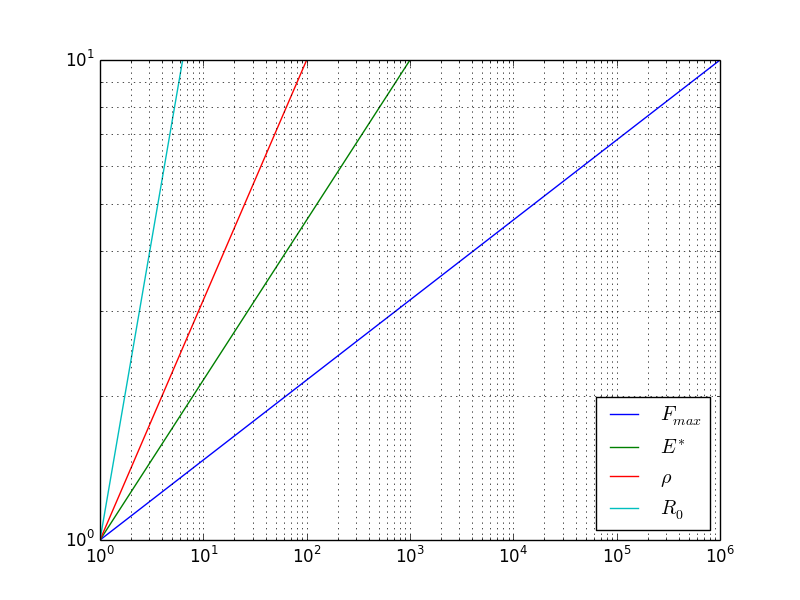
\includegraphics[width = 0.75 \textwidth]{chapters/figures/stability_curves}
% \caption{Curves showing the rate of response to timestep on the various normal-contact parameters.}\label{fig:stability-curves}
% \end{figure}

% It is apparent that simulations become less stable primarily as the pebble diameter decreases and then slightly less so for decreasing density and increasing the effective Young's modulus. It takes a rather large increase in the maximum contact force to cause the stable timestep to decrease. This is a fortunate result as it is primarily material properties which dictate stability of a DEM simulation. If external pressures increase and cause increases in the maximum normal contact force in the ensemble, it is unlikely to cause instabilities in the model. The result also provides insight into scaling of physical parameters to allow larger timesteps and thereby shorter overall duration of simulations.

The ceramic materials identified for breeders have relatively high Young's moduli, on the order of \si{10^{10} Pa}. The smallest radius will be on the order of \si{10^{-4} m}. The ceramic density is approximately on the scale of \si{10^{4} kg/m^3}. These values lead to a necessary timestep of

\begin{equation}
	\delta t_c \propto 10^{-7} \si{s}
\end{equation}

For a simulation that may last several hundreds of seconds of real time, this then requires more than 10$^9$ timesteps. If we have 10$^4$ particles in the simulation, each having their position integrated over a billion times, it becomes obvious that computational time is a major issue for our simulations of nuclear heating of ceramic breeder pebbles. If we are able to reduce the critical timestep (while perhaps decreasing the simulation time), the simulations will be much more practical for research use.
%~~~~~~~~~~~~~~~~~~~~~~~~~~~~~~~~~~~~~~~~~~~~~~~~~~~~~~~~~~~~~~~~~~~~~~~~~~~~~~~~




%~~~~~~~~~~~~~~~~~~~~~~~~~~~~~~~~~~~~~~~~~~~~~~~~~~~~~~~~~~~~~~~~~~~~~~~~~~~~~~~~
\subsection{Critical thermal timestep}

In \S\ref{sec:ht-pebble-conduction}, we introduced the dynamics of heat transfer between contacting particles in an ensemble. As we integrate the energy of an individual particle in time, we must also ensure that energy would not propagate through a particle faster than a single timestep can capture. In analogy to the critical timestep for mechanical stability (e.g. Eq.\ref{eq:rayleigh-stability-time}), we write for particle $i$,

\begin{equation}
	\delta t_\Bi = \frac{\rho_i C_i V_i}{H_c}
\end{equation}

where $\rho_i C_i V_i$ represents the inertial resistance to changing the temperature of $T_i$ and the conductance, $H_c$ represents the speed at which energy is delivered to $T_i$ from contact conduction. Then from the definition of $H_c$ we have given for smooth elastic spheres, this is also written as

\begin{equation}
	\delta t_\Bi = \frac{(4/3)\pi R_i^2\rho_i C_i}{2k^*}\frac{R_i}{a}
\end{equation}

For the material properties of lithium ceramics, as discussed for mechanical stability, we can expect

\begin{equation*}
	\frac{(4/3)\pi R_i^2\rho_i C_i}{2k^*} \approx \frac{(10^{-4})^210^{4}10^3}{10^0} = 10^{-1}
\end{equation*}

But from the requirements on Hertz theory in \S\ref{sec:hertz-contact}, we have required that $\frac{a}{R_i} \ll 1$. Thus the timestep for stability in the energy calculation is utterly negligible compared to the mechanical stability.

Vargas and McCarthy\cite{Vargas2001} make similar arguments, giving the criteria as,

\begin{equation}
	\frac{\mathrm{d}T_i}{T_i - T_j} \ll 1
\end{equation}

and too note that the timestep requirement for thermal calculations are orders of magnitude less restrictive than the analogous restriction of the particle dynamics.

Thus we can be confident that any timestep chosen for dynamic stability in the DEM simulation will automatically satisfy the timestep for thermal stability. 
%~~~~~~~~~~~~~~~~~~~~~~~~~~~~~~~~~~~~~~~~~~~~~~~~~~~~~~~~~~~~~~~~~~~~~~~~~~~~~~~~





%~~~~~~~~~~~~~~~~~~~~~~~~~~~~~~~~~~~~~~~~~~~~~~~~~~~~~~~~~~~~~~~~~~~~~~~~~~~~~~~~
\subsection{Simulation acceleration with scaled material properties}

We rewrite Eq.~\ref{eq:rayleigh-timestep} to facilitate a discussion on the parameters. Isolating each material term (neglecting the Poisson ratio) gives, 

\begin{equation}
	\delta t_c \propto R_i \times \rho_i^{1/2} \times E_i^{-1/2}
\end{equation}

% [pretty sure the approximation for $\nu$ only works when it's less than 1 so can't scale. must find out for sure.]

% The most direct effect would come from scaling the radius 





% From Makse\cite{Makse2004}

% We choose the time step to be a fraction of the time that it takes for a sound wave to propagate on the grain. Moreover, the quasistatic approximation used to calculate the Hertz force is valid only when the relative velocities of the par- ticles is smaller than the speed of sound in the grains\cite{Brilliantov1996}. Thus the characteristic time is $t_0 = R\sqrt{\rho_r/\mu_r}$ Typically, one chooses a time interval much smaller than the characteristic time, then $\Delta t=aR \sqrt{\rho_r/\mu_r}$ with $a<1$. Typical values for glass beads are:
% \si{\rho =2600 kg/m^3}, \si{\mu_r = 29 GPa}, \si{R = 0.1 mm}. Then $\Delta t$ should be smaller than \si{10^{−8} s}. Thus in order to perform a simulation over one second, more than $10^8$ steps are needed, which is obviously a very intensive computation. In this case, it is customary to increase the density or decrease the rigidity of the particles to allow for a larger time step to integrate the equations of motion over realistic periods of time. If the shear modulus of the grains in decreased, then it should be checked that the resulting stresses are several order of magnitude smaller than $\mu_r$, thus ensuring the condition of a nearly rigid system even though $\mu_r$ is taken smaller to obtain larger timesteps.

\section{Pebble failure modeling}
\label{failureDiscussion}
%In modeling pebble failure, there are two main tasks. The first is to develop a model for predicting a pebble failure event; { i.e.} what load (mechanical or thermal) will cause a pebble to crack, shatter, fracture, etc. The second is to develop a model which simulates the failure of that pebble; { i.e.} a scheme to treat a cracked, shattered, or crushed pebble in the assembly. 

The discrete element method has been used for studies in a variety of fields for studying inter-particle forces and the homogeneously distributed force networks that arise in packed beds (for example, see Ref.~\cite{Makse2000}). The discrete element method was also used in the fusion community to attempt to model failure initiation and propagation\cite{Annabattula2012a, Zhao2012, Zhao2013}. They too observed that a relatively few number of high-force networks, distributed troughought the bed supported the external mechanical loads. The even distribution of the force networks was used to defend the development of a probability-based predictor for failure. We make use of the probability argument of Zhao, {et al.} for the current study\cite{Zhao2013}. Their basic premise is that probability distributions of strength curves for pebble crushing have been observed (see, for example crush loads of Ref.~\cite{Tsuchiya1998}). Then in DEM models, a probability distribution of inter-particle forces are also observed. Overlaying the two probabilities resulted in seemingly random locations of pebbles satisfying the failure criteria -- not strictly along the high-force chains running through packed beds.

We apply the theory of Zhao, { et al.} in the following manner. If pebbles fail at random locations, we may de-couple the task of predicting pebble failure ({ i.e.} finding the mechanical or thermal load that causes a pebble to fail) from the task of modeling the ramifications of pebble failure. In our model, we begin with a starting point of a packed bed and then simply flag pebbles at random for `failing'. For our first model of failure, after a pebble has been flagged it is removed from the system entirely. The removal disrupts the meta-static state of the ensemble and the remaining pebbles re-settle. In reality, the ceramic pebbles generally break into just a few large pieces that remain in the system. Under development is a method for recreating that behavior in the DEM domain, it will be reported in future studies.

%Experiments on crushing single, brittle pebbles reveal that there are a number of failure modes\cite{Wu2004}. At one end, the pebble may simply crack and continue to hold a load for some time. At the other extreme, a pebble may crush virtually into a dust. We concern ourselves with the latter for this study. When a pebble in our simulation has been flagged for failure, we remove the pebble completely from the ensemble and then allow the remaining pebbles to rearrange to compensate for the lack of equilibrium on their contact forces. 


%\section{Simulation methods}
%\label{back} 
\section{DEM solver}\label{sec:dem-solver}

\subsection{Numerical Implementation Overview}

The primary computational tools used in this study is LAMMPS (Large-scale Atomic/Molecular Massively Parallel Simulator)\cite{Plimpton1995}; a classical molecular dynamics code. The package of code, maintained by Sandia National Labs (http://lammps.sandia.gov), has many features making it particularly attractive for our use on the simulation of pebble beds. LAMMPS is open-source and written in highly-portable C++ allowing customization of any feature used in modeling. LAMMPS runs with distributed-memory message-passing parallelism (MPI) and provides simple control (manual or automatic) of the spatial-decomposition of simulation domains for parallelizing. Perhaps most importantly, LAMMPS provides an efficient method for detecting and calculating pair-wise interaction forces; the largest consumer of run-time in the DEM algorithm\cite{Plimpton1995}. We build the code as a library so that LAMMPS can be coupled to other numerical tools; we use the scripting language of Python (Python 2.7) as an umbrella code to call LAMMPS routines with the full availability of Python libraries. 

LAMMPS by default provides a rudimentary method of modeling of granular particles (the term `granular' here differentiates the `discrete element' of molecules or atoms from larger-scale granular particles of powders or pebbles); LAMMPS has been used for studying granular material since at least 2001 when Silbert, et al.\cite{Silbert2001} studied granular flow on inclined planes. However, the usefulness of LAMMPS for studying granular systems was greatly enhanced by LIGGGHTS (LAMMPS Improved for General Granular and Granular Heat Transfer Simulations), a suite of modules included on top of LAMMPS. LIGGGHTS has many academic and industrial contributors from around the world, with the code maintained as open-source by DCS Computing, GmbH.

Briefly, some notable features the LIGGGHTS code brings to the LAMMPS environment include: Hertz/Hooke pair styles with shear history, mesh import for handling wall geometry, moving meshes, stress analysis of imported meshes, a macroscopic cohesion model, a heat transfer model, and improved dynamic load balancing of particles on processors\cite{Kloss2011}. Both LIGGGHTS and LAMMPS are distributed under the open-source codes under terms of the Gnu General Public License.

We will review some of the important physical models used in LAMMPS/LIGGGHTS as they relate to the important features we wish to investigate for packed beds of pebbles in fusion reactors.

\subsection{other solver info}

Time-discretization of the integration of Eq.~\ref{eq:newtons-second} is handled by the core Large-scale Atomic/Molecular Massively Parallel Simulator (LAMMPS) code released by Sandia National Laboratories\cite{Plimpton1995}. The code calculates velocity and position via the semi-explicit velocity-Verlet integration. The algorithm is stable with a global error of approximately $O(\Delta t^2)$ for displacement; details can be found in Ref.~\cite{Grubmuller1991}.

In the process of the study, to demonstrate the ability of the dynamic integration to capture resettling (and any possibly asymmetries), some beds were generated wherein the failure of pebbles was slightly localized near one or both $x$-walls. The profile of the pebbles near the top of the stack, after resettling, are shown in Fig.~\ref{fig:settlingStudy}. 

In our work, we occasionally required a fully quiesced bed. To determine when this occurred, the total kinetic energy of the entire ensemble was monitored and a packed bed was considered to have completely settled once the kinetic energy of the system was less than $10^{-9}$; similar to the process described in Ref.~\cite{Silbert2002}. 


The granular heat transfer equations are layered onto the LAMMPS code via a package of code named LIGGGHTS (LAMMPS Improved for General Granular and Granular Heat Transfer Simulations \cite{Kloss2012}). Parallelization of the code is straightforward with LAMMPS and we run the code on 128 nodes of UCLA's Hoffman2 cluster for typical run times of 18 to 24 hours per routine ({e.g.} filling, packing, heating, etc.).



